\subsection{1b}

\lstinputlisting{p1b.py}

As I have already explained that my rng is likely wrong, I will not mention
it further in the exercise. Here we use the Box-Muller method to generate
a Gaussian distribution, seen in \autoref{plt4}.
\begin{figure}[h!]
    \centering
    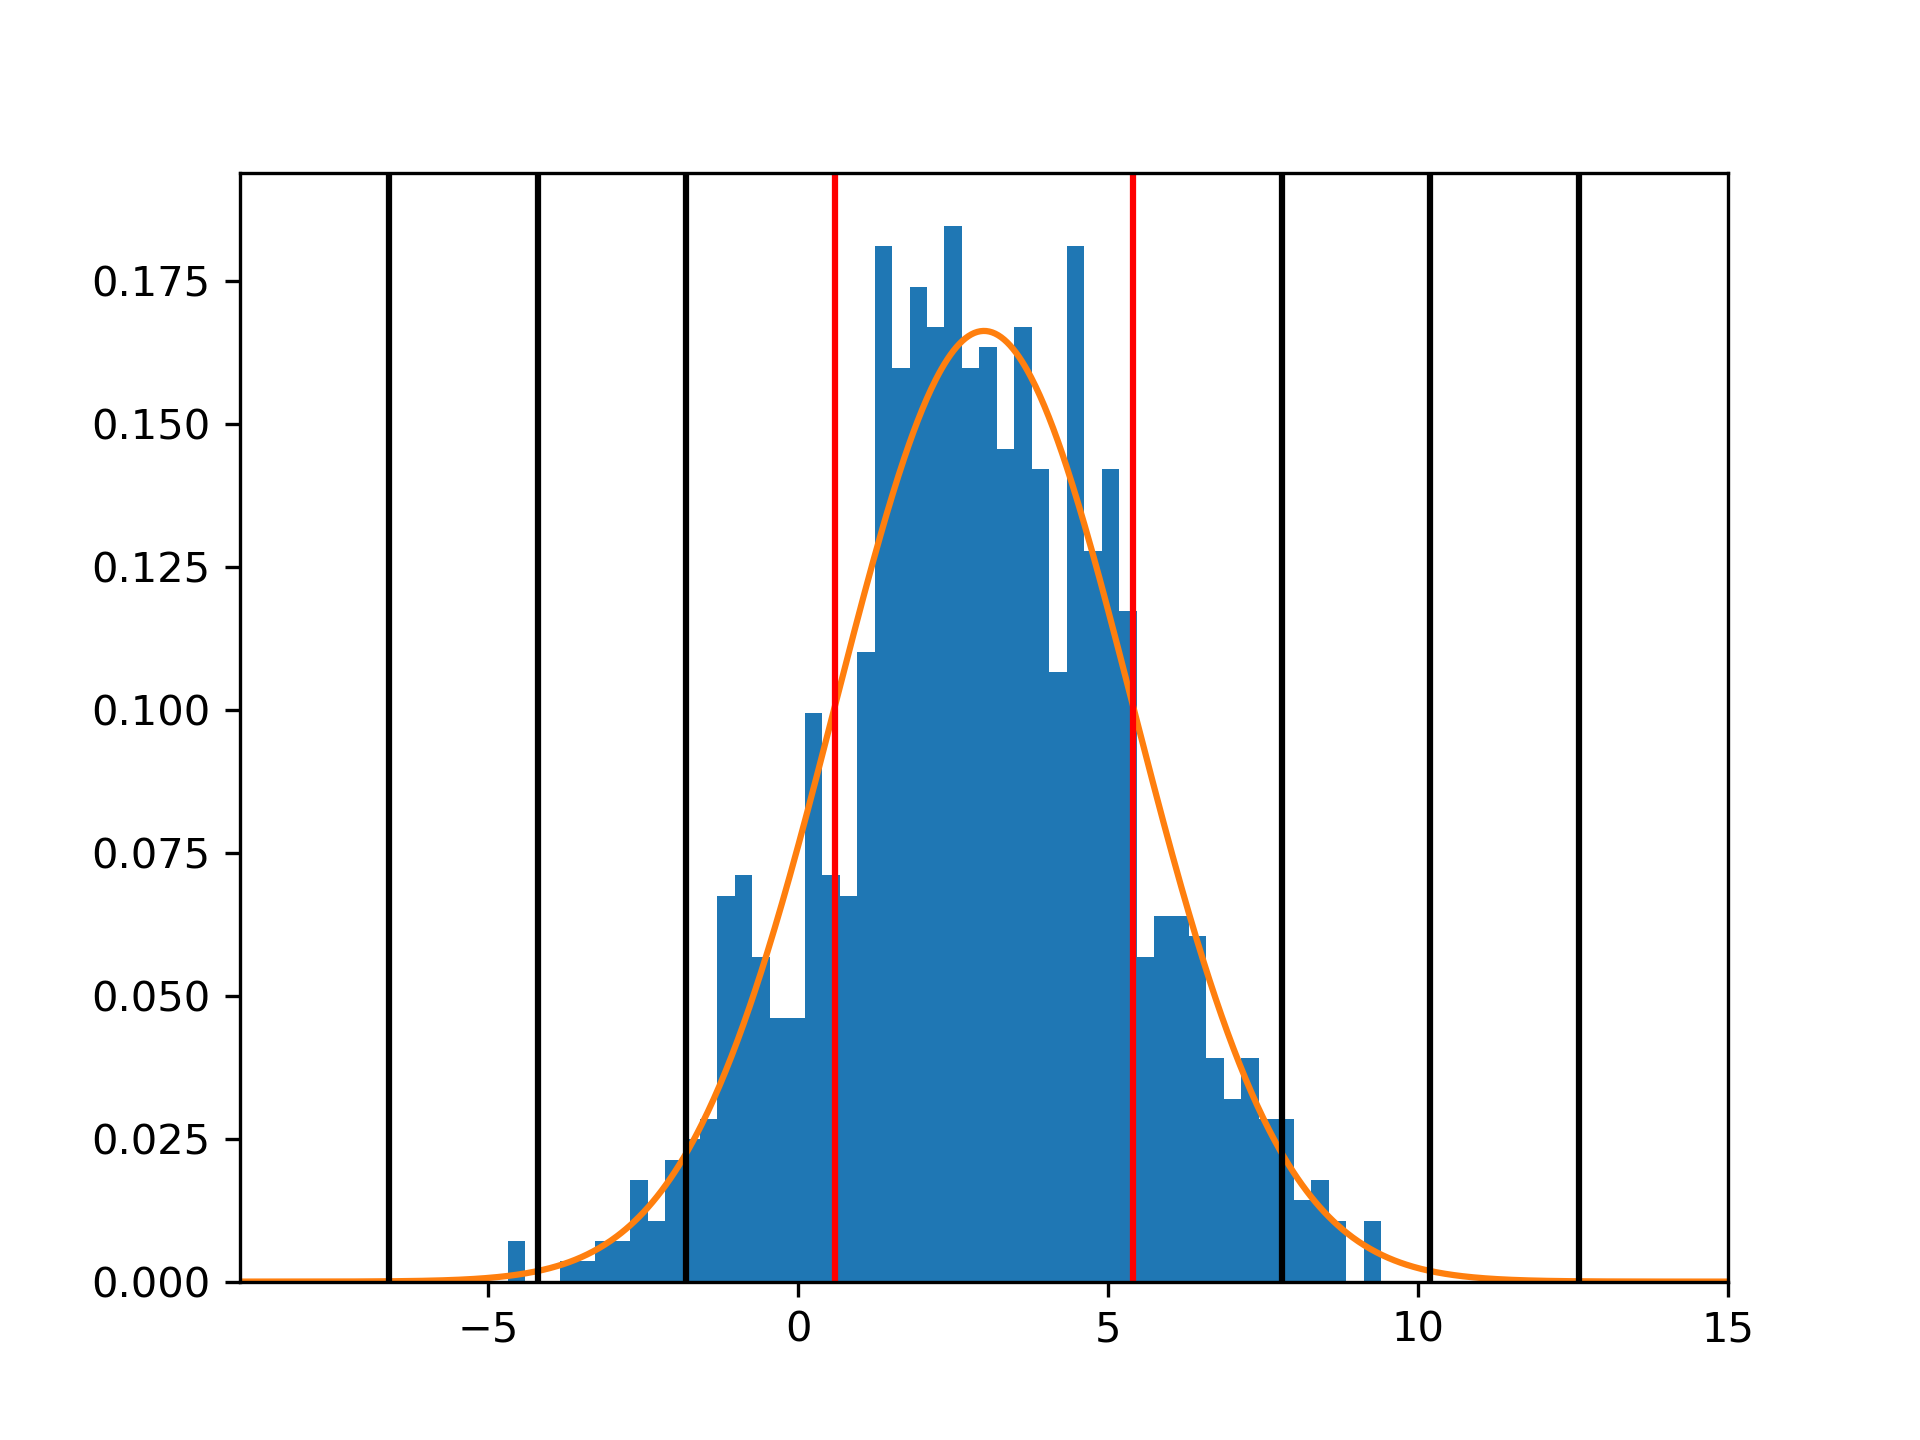
\includegraphics[width=0.9\linewidth]{./plots/box_gauss.png}
    \caption{My distribution with \texttt{numpy.norm} overplotted.}
    \label{plt4}
\end{figure}
The Box-Mueller method seems to work nicely, it is simply the rng that
ruins the Gaussian, given that there are values that are favored in the
$+1\sigma$ range.
